\documentclass[a4paper, 12pt]{article}

\usepackage[utf8]{inputenc}
\usepackage{amsmath}

\usepackage[]{amsfonts}
\usepackage[]{graphicx}

\title{CS231A Course Notes 4: Stereo Systems and Structure from Motion}
\author{Kenji Hata and Silvio Savarese}
\date{}

\renewcommand\emph{\textbf}

\numberwithin{equation}{section}
\begin{document}

\maketitle

\section{Introduction}
In the previous notes, we covered how adding additional viewpoints of a scene can greatly enhance our knowledge of the said scene. We focused on the epipolar geometry setup in order to relate points of one image plane to points in the other without extracting any information about the 3D scene. In these lecture notes, we will discuss how to recover information about the 3D scene from multiple 2D images.

\section{Triangulation}
One of the most fundamental problems in multiple view geometry is the problem of \emph{triangulation}, the process of determining the location of a 3D point given its projections into two or more images. 

\begin{figure}[h!]
\centering
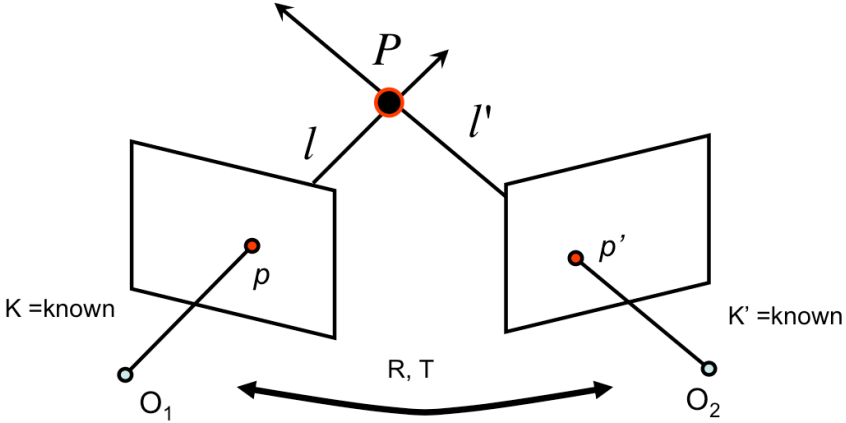
\includegraphics[width=0.8\textwidth]{figures/triangulation.png}
\caption{The setup of the triangulation problem when given two views.}
\label{fig:triangulation}
\end{figure}

In the triangulation problem with two views, we have two cameras with known camera intrinsic parameters $K$ and $K'$ respectively. We also know the relative orientations and offsets $R,T$ of these cameras with respect to each other. Suppose that we have a point $P$ in 3D, which can be found in the images of the two cameras at $p$ and $p'$ respectively. Although the location of $P$ is currently unknown, we can measure the exact locations of $p$ and $p'$ in the image. Because $K, K', R, T$ are known, we can compute the two lines of sight $\ell$ and $\ell'$, which are defined by the camera centers $O_1, O_2$ and the image locations $p, p'$. Therefore, $P$ can be computed as the intersection of $\ell$ and $\ell'$. 

\begin{figure}[h!]
\centering
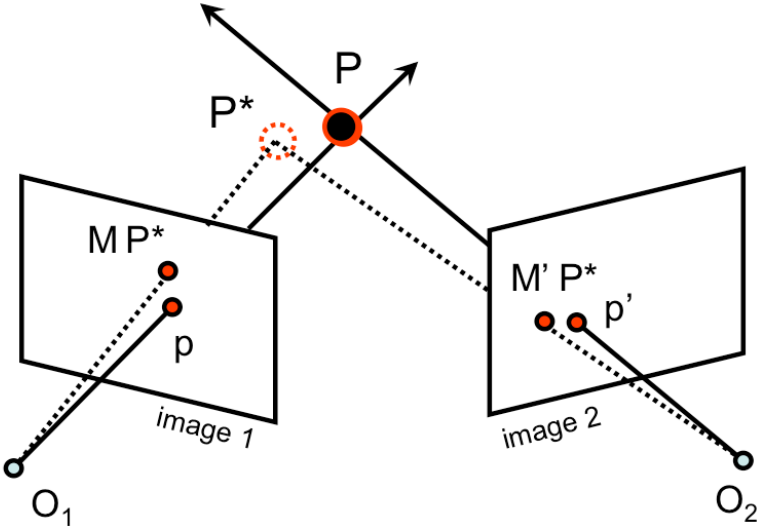
\includegraphics[width=0.8\textwidth]{figures/real_triangulation.png}
\caption{The triangulation problem in real-world scenarios often involves minimizing the reprojection error.}
\label{fig:real_triangulation}
\end{figure}

Although this process appears both straightforward and mathematically sound, it does not work very well in practice. In the real world, because the observations $p$ and $p'$ are noisy and the camera calibration parameters are not precise, finding the intersection point of $\ell$ and $\ell'$ may be problematic. In most cases, it will not exist at all, as the two lines may never intersect. 

\subsection{A linear method for triangulation}
In this section, we describe a simple linear triangulation method that solves the lack of an intersection point between rays. We are given two points in the images that correspond to each other $p = MP = (x,y,1)$ and $p'=M'P = (x', y', 1)$. By the definition of the cross product, $p\times(MP) = 0$. We can explicitly use the equalities generated by the cross product to form three constraints:
\begin{equation}
    \begin{split}
        x(M_3P) - (M_1P) = 0\\
        y(M_3P) - (M_2P) = 0\\
        x(M_2P) - y(M_1P) = 0
    \end{split}
\end{equation}
where $M_i$ is the $i$-th row of the matrix $M$. Similar constraints can be formulated for $p'$ and $M'$. Using the constraints from both images, we can formulate a linear equation of the form $AP = 0$ where
\begin{equation}
    A = \begin{bmatrix}
        xM_3 - M_1 \\ 
        y M_3 - M_2 \\
        x'M'_3 - M'_1 \\
        y'M'_3 - M'_2
    \end{bmatrix}
\end{equation}
This equation can be solved using SVD to find the best linear estimate of the point $P$. Another interesting aspect of this method is that it can actually handle triangulating from multiple views as well. To do so, one simply appends additional rows to $A$ corresponding to the added constraints by the new views.

This method, however is not suitable for projective reconstruction, as it is not projective-invariant. For example, suppose we replace the camera matrices $M, M'$ with ones affected by a projective transformation $MH^{-1}, M'H^{-1}$. The matrix of linear equations $A$ then becomes $AH^{-1}$. Therefore, a solution $P$ to the previous estimation of $AP=0$ will correspond to a solution $HP$ for the transformed problem $(AH^{-1})(HP) = 0$. Recall that SVD solves for the constraint that $\|P\| = 1$, which is not invariant under a projective transformation $H$. Therefore, this method, although simple, is often not the optimal solution to the triangulation problem. 
-
\subsection{A nonlinear method for triangulation}
Instead, the triangulation problem for real-world scenarios is often mathematically characterized as solving a minimization problem:
\begin{equation}
    \min_{\hat{P}} \|M\hat{P}-p\|^2 + \|M'\hat{P}-p'\|^2
    \label{eq:reprojection_error}
\end{equation}
In the above equation, we seek to find a $\hat{P}$ in 3D that best approximates $P$ by finding the best least-squares estimate of the \emph{reprojection error} of $\hat{P}$ in both images. The reprojection error for a 3D point in an image is the distance between the projection of that point in the image  and the corresponding observed point in the image plane. In the case of our example in Figure~\ref{fig:real_triangulation}, since $M$ is the projective transformation from 3D space to image 1, the projected point of $\hat{P}$ in image 1 is $M\hat{P}$. The matching observation of $\hat{P}$ in image 1 is $p$. Thus, the reprojection error for image 1 is the distance $\|M\hat{P} - p\|$. The overall reprojection error found in Equation~\ref{eq:reprojection_error} is the sum of the reprojection errors across all images. For cases with more than two images, we would simply add more distance terms to the objective function:
\begin{equation}
    \min_{\hat{P}} \sum_i \|M\hat{P_i}-p_i\|^2
    \label{eq:reprojection_error_multi_camera}
\end{equation}

In practice, there exists a variety of very sophisticated optimization techniques that result in good approximations to the problem. However, for the scope of the class, we will focus on only one of these techniques, which is the Gauss-Newton algorithm for nonlinear least squares. The general nonlinear least squares problem is to find an $x\in \mathbb{R}^n$ that minimizes
\begin{equation}
    \|r(x)\|^2 = \sum_{i=1}^m r_i(x)^2
\end{equation}
where $r$ is any residual function $r:\mathbb{R}^n\rightarrow \mathbb{R}^m$ such that $r(x) = f(x) - y$ for some function $f$, input $x$, and observation $y$. The nonlinear least squares problem reduces to the regular, linear least squares problem when the function $f$ is linear. However, recall that, in general, our camera matrices are not affine. Because the projection into the image plane often involves a division by the homogeneous coordinate, the projection into the image is generally nonlinear.

Notice that if we set $e_i$ to be a $2\times1$ vector $e_i = M\hat{P}_i - p_i$, then  we can reformulate our optimization problem to be:
\begin{equation}
    \min_{\hat{P}} \sum_i e_{i}(\hat{P})^2 
\end{equation}
which can be perfectly represented as a nonlinear least squares problem. 

In these notes, we will cover how we can use the popular Gauss-Newton algorithm to find an approximate solution to this nonlinear least squares problem. First, let us assume that we have a somewhat reasonable estimate of the 3D point $\hat{P}$, which we can compute by the previous linear method. The key insight of the Gauss-Newton algorithm is to update our estimate by correcting it towards an even better estimate that minimizes the reprojection error.  At each step we want to update our estimate $\hat{P}$ by some $\delta_P$: $\hat{P} = \hat{P} + \delta_P$.

But how do we choose the update parameter $\delta_P$? The key insight of the Gauss-Newton algorithm is to linearize the residual function near the current estimate $\hat{P}$. In the case of our problem, this means that the residual error $e$ of a point $P$ can be thought of as:
\begin{equation}
    e(\hat{P} + \delta_P) \approx e(\hat{P}) + \frac{\partial e}{\partial P}\delta_P
\end{equation}
Subsequently, the minimization problem transforms into
\begin{equation}
    \min_{\delta_P} \| \frac{\partial e}{\partial P}\delta_P - (-e(\hat{P})) \|^2
\end{equation}
When we formulate the residual like this, we can see that it takes the format of the standard linear least squares problem. For the triangulation problem with $N$ images, the linear least squares solution is
\begin{equation}
    \delta_P = -(J^TJ)^{-1} J^Te
\end{equation}
where 
\begin{equation}
    e = \begin{bmatrix} e_1 \\ \vdots \\ e_N\end{bmatrix} = \begin{bmatrix}p_1 - M_1\hat{P} \\ \vdots \\ p_n - M_n \hat{P} \end{bmatrix}
\end{equation}
and
\begin{equation}
    J = \begin{bmatrix}
    \dfrac{\partial e_1}{\partial \hat{P}_1} & \dfrac{\partial e_1}{\partial \hat{P}_2}& \dfrac{\partial e_1}{\partial \hat{P}_3}\\
    \vdots & \vdots & \vdots\\
    \dfrac{\partial e_N}{\partial \hat{P}_1} & \dfrac{\partial e_N}{\partial \hat{P}_2} & \dfrac{\partial e_N}{\partial \hat{P}_3} \end{bmatrix}
\end{equation}
 
 Recall that the residual error vector of a particular image $e_i$ is a $2\times 1$ vector because there are two dimensions in the image plane. Consequently, in the simplest two camera case ($N=2$) of triangulation, this results in the residual vector $e$ being a $2N\times1 = 4\times1$ vector and the Jacobian $J$ being a $2N\times3 =4 \times 3$ matrix. Notice how this method handles multiple views seamlessly, as additional images are accounted for by adding the corresponding rows to the $e$ vector and $J$ matrix. After computing the update $\delta_P$, we can simply repeat the process for a fixed number of steps or until it numerically converges. One important property of the Gauss-Newton algorithm is that our assumption that the residual function is linear near our estimate gives us no guarantee of convergence. Thus, it is always useful in practice to put an upper bound on the number of updates made to the estimate.

\section{Affine structure from motion}
At the end of the previous section, we hinted how we can go beyond two views of a scene to gain information about the 3D scene. We will now explore the extension of the geometry of two cameras to multiple cameras. By combining observations of points from multiple views, we will be able to simultaneously determine both the 3D structure of the scene and the parameters of the camera in what is known as \emph{structure from motion}.

\begin{figure}[h!]
\centering
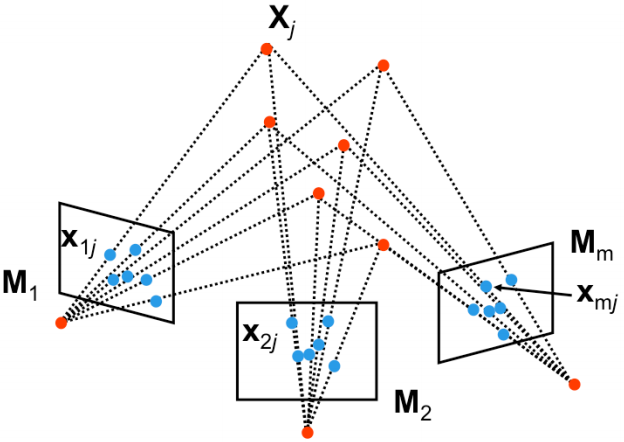
\includegraphics[width=0.8\textwidth]{figures/sfm_setup.png}
\caption{The setup of the general structure from motion problem.}
\label{fig:sfm_setup}
\end{figure}

Here, we formally introduce the structure from motion problem. Suppose we have $m$ cameras with camera transformations $M_i$ encoding both the intrinsic and extrinsic parameters for the cameras. Let $X_j$ be one of the $n$ 3D points in the scene. Each 3D point may be visible in multiple cameras at the location $x_{ij}$, which is the projection of $X_j$  to the image of the camera $i$ using the projective transformation $M_i$. The aim of structure from motion is to recover both the structure of the scene (the $n$ 3D points $X_j$) and the motion of the cameras (the $m$ projection matrices $M_i$) from all the observations $x_{ij}$. 

\subsection{The affine structure from motion problem}
Before tackling the general structure from motion problem, we will first start with a simpler problem, which assumes the cameras are affine or weak perspective. Ultimately, the lack of the perspective scaling operation makes the mathematical derivation easier for this problem. 

Previously, we derived the above equations for perspective and weak perspective cases. Remember that in the full perspective model, the camera matrix is defined as 
\begin{equation}
M = \begin{bmatrix}
    A & b \\ v & 1
\end{bmatrix}    
\end{equation}
where $v$ is some non-zero $1\times3$ vector. On the other hand, for the weak perspective model, $v=0$. We find that this property makes the homogeneous coordinate of $MX$ equal to $1$: 
\begin{equation}
    x = MX = \begin{bmatrix}m_1 \\ m_2 \\ 0 ~~ 0 ~~ 0 ~~ 1\end{bmatrix} \begin{bmatrix}X_1\\X_2\\X_3 \\ 1\end{bmatrix} = \begin{bmatrix}m_1X \\ m_2 X \\ 1\end{bmatrix}
\end{equation}

Consequently, the nonlinearity of the projective transformation disappears as we move from homogeneous to Euclidean coordinates, and the weak perspective transformation acts as a mere magnifier. We can more compactly represent the projection as:
\begin{equation}
    \begin{bmatrix} m_1X \\ m_2X \end{bmatrix} = \begin{bmatrix}A & b \end{bmatrix} X = AX + b
\end{equation}
and represent any camera matrix in the format $M_\mathrm{affine} = \begin{bmatrix}A &b \end{bmatrix}$. Thus, we now use the affine camera model to express the relationship from a point $X_j$  in 3D and the corresponding observations in each affine camera (for instance, $x_{ij}$ in camera $i$).

Returning to the structure from motion problem, we need to estimate $m$ matrices $M_i$, and the $n$ world coordinate vectors $X_j$, for a total of $8m+3n$ unknowns, from $mn$ observations. Each observation creates 2 constraints per camera, so there are $2mn$ equations in $8m+3n$ unknowns. We can use this equation to know the lower bound on the number of corresponding observations in each of the images that we need to have. For example, if we have $m=2$ cameras, then we need to have at least $n=16$ points in 3D. However, once we do have enough corresponding points labeled in each image, how do we solve this problem?  

\subsection{The Tomasi and Kanade factorization method} 
In this part, we outline Tomasi and Kanade’s \emph{factorization method} for solving the affine structure from motion problem. This method consists of two major steps: the data centering step and the actual factorization step. 

\begin{figure}[h!]
\centering
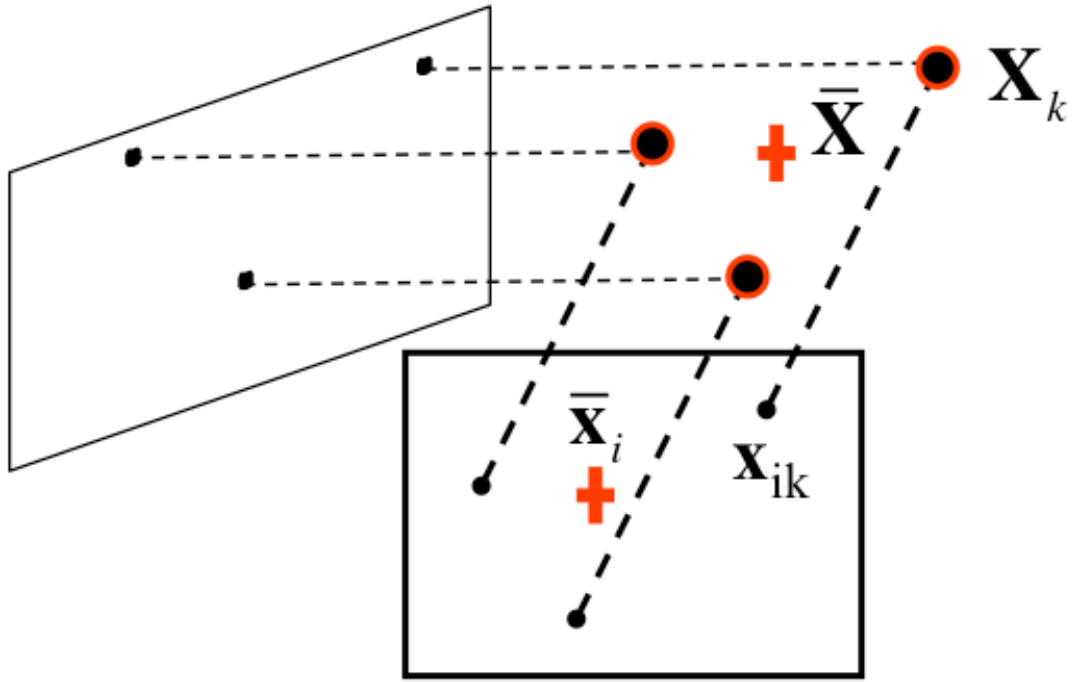
\includegraphics[width=0.8\textwidth]{figures/factorization_centering.png}
\caption{When applying the centering step, we translate all of the image points such that their centroid (denoted as the lower left red cross) is located at the origin in the image plane. Similarly, we place the world coordinate system such that the origin is at the centroid of the 3D points (denoted as the upper right red cross).}
\label{fig:factorization_centering}
\end{figure}

Let’s begin with the data centering step. In this step, the main idea is center the data at the origin. To do so, for each image $i$, we redefine new coordinates $\hat{x}_{ij}$ for each image point $x_{ij}$ by subtracting out their centroid $\bar{x}_i$:
\begin{equation}
    \hat{x}_{ij} = x_{ij} - \bar{x}_{i} = x_{ij} - \frac{1}{n}\sum_{j=1}^{n}{x_{ij}}
    \label{eq:mean}
\end{equation}
Recall that the affine structure from motion problem allows us to define the relationship between image points $x_{ij}$, the camera matrix variables $A_i$ and $b_i$, and the 3D points $X_j$ as:
\begin{equation}
    x_{ij}= A_i X_j + b_i
    \label{eq:affine_relationship}
\end{equation}
After this centering step, we can combine definition of the centered image points $\hat{x}_{ij}$ in Equation~\ref{eq:mean} and the affine expression in Equation~\ref{eq:affine_relationship}:
\begin{equation}
\begin{split}
    \hat{x}_{ij} &= x_{ij} -  \frac{1}{n}\sum_{k=1}^{n}{x_{ik}}\\
    & = A_iX_j - \frac{1}{n}\sum_{k=1}^{n}{A_i X_k}\\
    & = A_i(X_j - \frac{1}{n}\sum_{k=1}^{n} X_k) \\ 
    & = A_i(X_j - \bar{X})\\
    & = A_i\hat{X}_j
\end{split}
\label{eq:centered_relationship}
\end{equation}

As we see from Equation~\ref{eq:centered_relationship}, if we translate the origin of the world reference system to the centroid $\bar{X}$, then the centered coordinates of the image points $\hat{x}_{ij}$ and centered coordinates of the 3D points $\hat{X}_{ij}$ are related only by a single $2\times 3$ matrix $A_i$. Ultimately, the centering step of the factorization method allows us to create a compact matrix product representation to relate the 3D structure with their observed points in multiple images.

However, notice that in the matrix product $\hat{x}_{ij} = A_i\hat{X_j}$, we only have access to the values on the left hand side of the equation. Thus, we must somehow factor out the motion matrices $A_i$ and structure $X_j$. Using all the observations for all the cameras, we can build a measurement matrix $D$, made up of $n$ observations in the $m$ cameras (remember that each $\hat{x}_{ij}$ entry is a 2x1 vector):
\begin{equation}
    D = \begin{bmatrix}
        \hat{x}_{11} & \hat{x}_{12} & \hdots & \hat{x}_{1n}\\
        \hat{x}_{2  1} & \hat{x}_{22} & \hdots & \hat{x}_{2n}\\
        & & \ddots & \\
        \hat{x}_{m1} & \hat{x}_{m2} & \hdots & \hat{x}_{mn}\\
    \end{bmatrix}
\end{equation}

Now recall that because of our affine assumption, $D$ can be expressed as the product of the $2m\times3$ motion matrix $M$ (which comprises the camera matrices $A_1, \ldots A_m$) and the $3\times n$ structure matrix $S$ (which comprises the 3D points $X_1, \ldots X_n$). An important fact that we will use is that $\mathrm{rank}(D) = 3$ since $D$ is the product of two matrices whose max dimension is 3. 

To factorize $D$ into $M$ and $S$, we will use the singular value decomposition, $D = U \Sigma V^T$. Since we know the $\mathrm{rank}(D) = 3$, so there will only be 3 non-zero singular values $\sigma_1 , \sigma_2$, and $\sigma_3$ in $\Sigma$. Thus, we can further reduce the expression and obtain the following decomposition:
\begin{equation}
    \begin{split}
        D &= U \Sigma V^T\\ 
        &= \begin{bmatrix} u_1 & \hdots & u_n \end{bmatrix} 
        \begin{bmatrix}
            \sigma_1 & 0 & 0 & 0 & \hdots & 0\\
            0 & \sigma_2 & 0 & 0 & \hdots & 0\\ 
            0 & 0 & \sigma_3 & 0 & \hdots & 0\\ 
            0 & 0 & 0 & 0 & \hdots & 0\\ 
             &  &  & & \ddots & \\ 
            0 & 0 & 0 & 0 & \hdots & 0\\ 
        \end{bmatrix}
        \begin{bmatrix} v_1^T \\ \vdots \\ v_n^T \end{bmatrix}\\
        & = \begin{bmatrix} u_1 & u_2 & u_3 \end{bmatrix} 
        \begin{bmatrix}
            \sigma_1 & 0 & 0\\
            0 & \sigma_2 & 0\\ 
            0 & 0 & \sigma_3
        \end{bmatrix}
        \begin{bmatrix} v_1^T \\ v_2^T \\ v_3^T \end{bmatrix}\\
        & = U_3 \Sigma_3 V^T_3
    \end{split}
    \label{eq:svd_factorization}
\end{equation}

In this decomposition, $\Sigma_3$ is defined as the diagonal matrix formed by the non-zero singular values, while $U_3$ and $V^T_3$ are obtained by taking the corresponding three columns of $U$ and rows of $V^T$ respectively. Unfortunately, in practice, $\mathrm{rank}(D) > 3$ because of measurement noise and the affine camera approximation. However, recall that when $\mathrm{rank}(D) > 3$, $U_3 W_3 V_3^T$ is still the best possible rank-3 approximation of $MS$ in the sense of the Frobenius norm. 

Upon close inspection, we see that the matrix product $\Sigma_3V_3^T$ forms a $3\times n$ matrix, which exactly the same size as the structure matrix $S$. Similarly, $U_3$ is a $2m\times 3$ matrix, which is the same size as the motion matrix $M$. While this way of associating the components of the SVD decomposition to $M$ and $S$ leads to a physically and geometrical plausible solution of the affine structure from motion problem, this choice is not a unique solution. For example, we could also set the motion matrix to $M = U_3\Sigma_3$ and the structure matrix to $S = V_3^T$, since in either cases the observation matrix $D$ is the same. So what factorization do we choose? In their paper, Tomasi and Kanade concluded that a robust choice of the factorization is $M = U_3\sqrt{\Sigma_3}$ and $S = \sqrt{\Sigma_3}V_3^T$.

\subsection{Ambiguity in reconstruction}
Nevertheless, we find inherent ambiguity in any choice of the factorization $D=MS$, as any arbitrary, invertible $3 \times 3$ matrix $A$ may be inserted into the decomposition:
\begin{equation}
    D = MAA^{-1}S = (MA)(A^{-1}S)
\end{equation}
This means that the camera matrices obtained from motion $M$ and the 3D points obtained from structure $S$ are determined up to a multiplication by a common matrix $A$. Therefore, our solution is underdetermined, and requires extra constraints to resolve this affine ambiguity. When a reconstruction has affine ambiguity, it means that parallelism is preserved, but the metric scale is unknown.

Another important class of ambiguities for reconstruction is the similarity ambiguity, which occurs when a reconstruction is correct up to a similarity transform (rotation, translation and  scaling). A reconstruction with only similarity ambiguity is known as a metric reconstruction. This ambiguity exists even when the camera are intrinsically calibrated.  The good news is that for calibrated cameras, the similarity ambiguity is the only ambiguity\footnote{See [Longuet-Higgins ’81] for more details.}. 

The fact that there is no way to recover the absolute scale of a scene from images is fairly intuitive. An object's scale, absolute position and canonical orientation will always be unknown unless we make further assumptions (e.g, we know the height of the house in the figure) or incorporate more data. This is because some attributes may compensate for others. For instance, to get the same image, we can simply move the object backwards and scale it accordingly. One such example of removing similarity ambiguity occurred during the camera calibration procedure, where we made the assumption that we know the location of the calibration points with respect to the world reference system. This enabled us to know the size of the squares of the checkerboard to learn a metric scale of the 3D structure.

\section{Perspective structure from motion}
After studying the simplified affine structure from motion problem, let us now consider the general case for projective cameras $M_i$. In the general case with projective cameras, each camera matrix $M_i$ contains 11 degrees of freedom, as it is defined up to scale:
\begin{equation}
M_i=
\begin{bmatrix}
    a_{11}       & a_{12} & a_{13} &  b_{1} \\
    a_{21}       & a_{22} & a_{23} &  b_{2} \\
    a_{31}       & a_{32} & a_{33} &  1
\end{bmatrix}
\end{equation}

Moreover, similar to the affine case where the solution can be found up to an affine transformation, solutions for structure and motion can be determined up a projective transformation in the general case: we can always arbitrarily apply a $4\times 4$ projective transformation $H$ to the motion matrix, as long as we also transform the structure matrix by the inverse transformation $H^{-1}$. The resulting observations in the image plane will still be the same.

Similar to the affine case, we can set up the general structure from motion problem as estimating both the $m$ motion matrices $M_i$ and $n$ 3D points $X_j$ from $mn$ observations $x_{ij}$. Because cameras and points can only be recovered up to a $4\times 4$ projective transformation up to scale (15 parameters), we have $11m+3n-15$ unknowns in $2mn$ equations. From these facts, we can determine the number of views and observations that are required to solve for the unknowns. 

\subsection{The algebraic approach}

\begin{figure}[h!]
\centering
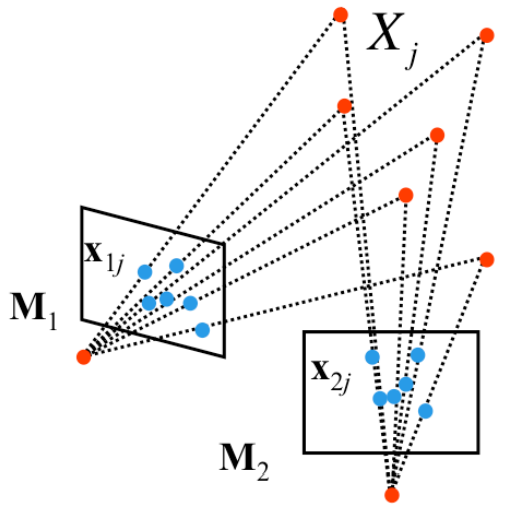
\includegraphics[width=0.5\textwidth]{figures/algebraic_setup.png}
\caption{In the algebraic approach, we consider sequential, camera pairs to determine camera matrices $M_1$ and $M_2$ up to a perspective transformation. We then find a perspective transformation $H$ such that $M_1H = [I~~0]$ and $M_2H = [A~~B]$}.
\label{fig:algebraic_setup}
\end{figure}

We will now cover the \emph{algebraic approach}, which leverages the concept of fundamental matrix $F$ for solving the structure from motion problem for two cameras. As shown in Figure~\ref{fig:algebraic_setup}, the main idea of the algebraic approach is to compute two camera matrices $M_1$ and $M_2$, which can only be computed up to a perspective transformation $H$. Since each $M_i$ can only be computed up a perspective transformation $H$, we can always consider a $H$ such that the first camera projection matrix $M_1 H^{-1}$ is canonical. Of course, the same transformation must also be applied to the second camera which lead to the form shown:

\begin{equation}
    M_1 H^{-1} = [I ~~ 0] ~~~~~~~ M_2 H^{-1} = [A ~~ b]
    \label{eq:mh}
\end{equation}

In order to accomplish this task, we must first compute the fundamental matrix $F$ using the eight point algorithm covered in the previous course notes. We now will use $F$ to estimate the projective camera matrices $M_1$ and $M_2$. In order to do this estimation, we define $P$ to be the corresponding 3D point for the corresponding observations in the images $p$ and $p'$. Since we have applied $H^{-1}$ to both camera projection matrices, we must also apply $H$ to the structure, giving us $\widetilde{P} = HP$. Therefore, we can relate the pixel coordinates $p$ and $p'$ to the transformed structure as follows:

\begin{equation}
    \begin{split}
        p = M_1 P = M_1 H^{-1} H P = [I ~ | ~ 0] \widetilde{P}\\
        p' = M_2 P = M_2 H^{-1} H P = [A ~ | ~ b] \widetilde{P}
    \end{split}
    \label{eq:x}
\end{equation}
An interesting property between the two image correspondences $p$ and $p'$ occur by some creative substitutions:

\begin{equation}
    \begin{split}
        p'&= [A|b] \widetilde{P}\\
        &= A[I|0] \widetilde{P} +b \\
        &= Ap+b
    \end{split}
    \label{eq:xpx}
\end{equation}
Using Equation~\ref{eq:xpx}, we can write the cross product between $p'$ and $b$ as:

\begin{equation}
    p' \times b = (Ap+b) \times b = Ap \times b 
    \label{eq:xptimesb}
\end{equation}
By the definition of cross product, $p' \times b$ is perpendicular to $p'$. Therefore, we can write:

\begin{equation}
    \begin{split}
        0 &= p'^T  ( p' \times b )  \\
        &= p'^T  (Ap \times b )\\
        &= p'^T \cdot (b \times Ap) \\
        & = p'^T[b]_\times Ap
    \end{split}
    \label{eq:xpdot1}
\end{equation}
Looking at this constraint, it should remind you of the general definition of the Fundamental matrix $p'^T Fp = 0$. If we set $F=[b]_\times A$, then extracting $A$ and $b$ simply breaks down to a decomposition problem. 

Let us begin by determining $b$. Again, by the definition of cross product, we can simply write $Fb$ as 
\begin{equation}
    Fb = [b]_\times A b = (b\times A)b = 0
    \label{eq:cross_b}
\end{equation}.  
Since $F$ is singular, $b$ can be computed as a least square solution of $F b = 0$, with $\|b\|=1$, using SVD. 

Once $b$ is known, we can now compute $A$. If we set $A=-[b]_\times F$, then we can verify that this definition satisfies $F = [b]_\times A$:
\begin{equation}
    \begin{split}
        [b_\times]A' &= -[b_\times][b_\times]F \\
        & =(bb^T - |b|^2I)F \\
        &= bb^TF + |b|^2F \\
        &= 0 + 1\cdot F \\
        &=F
    \end{split}
    \label{eq:bap}
\end{equation}
Consequently, we determine the two expressions for our camera matrices $M_1H^{-1}$ and $M_2H^{-1}$:
\begin{equation}
    \tilde{M}_1 = [I ~~ 0] ~~~~~~~~ \tilde{M}_2 = [- [b_\times]F ~~ b]
    \label{eq:mm}
\end{equation}

Before we conclude this section, we want give a geometrical interpretation for $b$. We know $b$ satisfies $Fb=0$. Remember the epipolar constraints we derived in the previous course notes, which found that the epipoles in an image are the points that map to zero when transformed by the Fundamental matrix (i.e. $Fe_2=0$ and $F^T e_1=0$). We can see, therefore, that $b$ is an epipole. This provides a new set of equations for the camera projection matrices (Eqs. \ref{eq:mm2}). 

\begin{equation}
    \tilde{M}_1 = [I ~~ 0] ~~~~~~~~ \tilde{M}_2 = [- [e_\times]F ~~ e]
    \label{eq:mm2}
\end{equation}

\subsection{Determining motion from the Essential matrix}
One useful way of improving the reconstruction obtained by the algebraic approach is to use calibrated cameras. We can extract a more accurate, initial estimate of camera matrices by using the Essential matrix, which is a special case of the Fundamental matrix for normalized coordinates. Recall that, by using the Essential matrix $E$, we make an assumption that we have calibrated the camera and thus know the intrinsic camera matrix $K$. We can either compute the Essential matrix $E$ either from the normalized image coordinates directly or from its relationship with the Fundamental matrix $F$ and intrinsic matrix $K$:

\begin{equation}
    E = K^TFK
\end{equation}

Because the Essential matrix assumes that we have calibrated cameras, we should remember that it only has five degrees of freedom, as it only encodes the extrinsic parameters: the rotation $R$ and translation $t$ between the cameras. Luckily, this is exactly the information that we want to extract to create our motion matrix. First, recall that the Essential matrix $E$ can be represented as
\begin{equation}
    E = [t]_\times R
\end{equation}
As such, perhaps we can find a strategy to factor $E$ into its two components. First, we should notice that the cross product matrix $[t]_\times$ is skew-symmetric. We define two matrices that we will use in the decomposition:
\begin{equation}
     W = \begin{bmatrix} 0 & -1 & 0 \\ 1 & 0 & 0 \\ 0 & 0 & 1\end{bmatrix}, ~~~ Z = \begin{bmatrix} 0 & 1 & 0 \\ -1 & 0 & 0 \\ 0 & 0 & 0\end{bmatrix}
\end{equation}
One important property we will use later is that $Z = \mathrm{diag}(1,1,0)W$ up to a sign. Similarly, we will also use the fact that $ZW = ZW^T = \mathrm{diag}(1,1,0)$ up to a sign. 

As a result of eigenvalue decomposition, we can create a block decomposition of a general skew-symmetric matrix known up to scale. Thus, we can write $[t]_\times$ as 
\begin{equation}
    [t]_\times  = UZU^T
\end{equation}
where $U$ is some orthogonal matrix. Therefore, we can rewrite the decomposition as:
\begin{equation}
    E = U\mathrm{diag}(1,1,0)  (WU^TR)
\end{equation}

Looking at this expression carefully, we see that it closely resembles the singular value decomposition $E = U\Sigma V^T$, where $\Sigma$ contains two equal singular values. If we know $E$ up to scale and we assume that it takes the form $E = U \mathrm{diag}(1,1,0)V^T$, then we arrive at the following factorizations of $E$:
\begin{equation}
    [t]_\times  = UZU^T, ~~~~ R= UWV^T ~ \mathrm{or} ~ UW^TV^T
\end{equation}
We can prove that the given factorizations are valid by inspection. We can also prove that there are no other factorizations. The form of $[t]_\times$ is determined by the fact that its left null space must be the same as the null space of $E$. Given unitary matrices $U$ and $V$, any rotation $R$ can be decomposed into $UXV^T$ where $X$ is another rotation matrix. After substituting these values in, we get $ZX = \mathrm{diag}(1,1,0)$ up to scale. Thus, $X$ must be equal to $W$ or $W^T$. 

Note that this factorization of $E$ only guarantees that the matrices $UWV^T$ or $UW^TV^T$ is orthogonal. To ensure that $R$ is a valid rotations, we simply make sure that the determinant of $R$ is positive:
\begin{equation}
    R= (\det UWV^T)UWV^T ~ \mathrm{or} ~ (\det UW^TV^T)UW^TV^T
\end{equation}

Similar to how the rotation $R$ can take on two potential values, the translation vector $t$ can also take on several values. From the definition of cross product, we know that
\begin{equation}
    t \times t = [t]_\times t = UZU^T t = 0
\end{equation}
Knowing that $U$ is unitary, we can find that the $\|[t]_\times\|_F = \sqrt{2}$. Therefore, our estimate of $t$ from this factorization will From the above equation and the fact that $E$ is known up to scale, this means that 
\begin{equation}
    t = \pm U\begin{bmatrix}0\\0\\1\end{bmatrix} = \pm u_3
\end{equation}
where $u_3$ is the third column of $U$. By inspection, we can also verify that we get the same results by reformatting $[t]_\times = UZU^T$ into the vector $t$ known up to a sign.

\begin{figure}[h!]
\centering
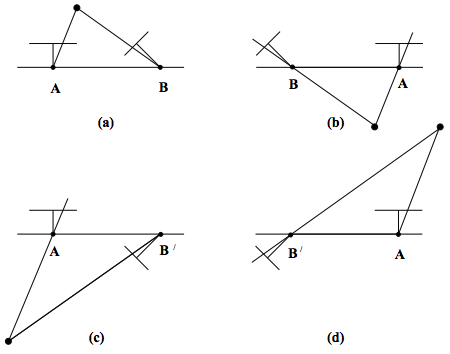
\includegraphics[width=0.8\textwidth]{figures/four_rt.png}
\caption{There are four possible solutions for extracting the relative camera rotation $R$ and translation $t$ from the Essential matrix. However, only in (a) is the reconstructed point in front of both of the cameras. (Figure taken from Hartley and Zisserman textbook page 260)}
\label{fig:four_rt}
\end{figure}

As illustrated in Figure~\ref{fig:four_rt}, there are four potential $R,t$ pairings since there exists two options for both $R$ and $t$. Intuitively, the four pairings include all possible pairings of rotating a camera in a certain direction or rotating the camera in the opposite direction combined with the option of translating it in a certain direction or the opposite direction. Therefore, under ideal conditions, we would only need to triangulate one point to determine the correct $R,t$ pair. For the correct $R,t$ pair, the triangulated point $\hat{P}$ exists in front of both cameras, which means that it has a positive $z$-coordinate with respect to both camera reference systems. Due to measurement noise, we often do not rely on triangulating only one point, but will instead triangulate many points and determine the correct $R,t$ pair as the one that contains the most of these points in front of both cameras.

\section{An example structure from motion pipeline}
After finding the relative motion matrices $M_i$, we can use them to determine the world coordinates of the points $X_j$. In the case of the algebraic method, the estimate of such points will be correct up the perspective transformation $H$. In the extracting the camera matrices from the Essential matrix, the estimates can be known up to scale. In both cases, the 3D points can be computed from the estimated camera matrices via the triangulation methods described earlier.

The extension to the multi-view case can be done by chaining pairwise cameras. We can use the algebraic approach or the Essential matrix to obtain solutions for the camera matrices and the 3D points for any pair of cameras, provided that there are enough point correspondences. The reconstructed 3D points are associated to the point correspondences available between the camera pair. Those pairwise solutions may be combined together (optimized) in a approach called bundle adjustment as we will see next.

\subsection{Bundle adjustment}
There are major limitations related to the previous methods for solving the structure from motion problem that we have discussed so far. The factorization method assumes that all points are visible in every image. This is very unlikely to happen because of occlusions and failures to find correspondences when we either have many images or some of the images were taken far apart. Finally the algebraic approach produces pairwise solutions that can be combined into a camera chain, but does not solve for a coherent optimized reconstruction using all the cameras and 3D points.

To address these limitations, we introduce \emph{bundle adjustment}, which is a nonlinear method for solving the structure from motion problem. In the optimization, we aim to minimize the reprojection error, which is the pixel distance between the projection of a reconstructed point into the estimated cameras and its corresponding observations for all the cameras and for all the points. Previously, when discussing nonlinear optimization methods for triangulation, we focused primarily on the two camera case, in which we naturally assumed that each camera saw all the correspondences between the two. However, since bundle adjustment handles several cameras, it only calculates the reprojection error for only the observations that can be seen by each camera. Ultimately though, this optimization problem is very similar to the one we introduced when talking about nonlinear methods for triangulation. 

Two common approaches for solving bundle adjustment's nonlinear optimization include the Gauss-Newton algorithm and the Levenberg-Marquardt algorithm. You can refer to the previous section about details on the Gauss-Newton algorithm and refer to the Hartley and Zisserman textbook for more details on the Levenberg-Marquardt algorithm.

In conclusion, bundle adjustment has some important advantages and limitations when compared to the other methods we have surveyed. It is particularly useful because it can handle a large number of views smoothly and also handle cases when particular points are not observable by every image. However, the main limitation is that it is a particularly large minimization problem, as the parameters grow with the number of views. Additionally, it requires a good initial condition since it relies on nonlinear optimization techniques. For this reason, bundle adjustment is often used as final step of most structure from motion implementations (i.e., after the factorization or algebraic approach), as a factorization or algebraic approach may provide a good initial solution for the optimization problem. 
\end{document}
